\section{Results}
\label{sec:results}

\subsection{Final numerical-reference run}

The finalized ANUGA run under the all-reflective policy completed in
57.0764~s and produced 61 processed output times.  Its maximum absolute
mass-balance error was \(7.23468\times10^{-5}\)~m\(^3\), corresponding to a
maximum relative error of \(8.52467\times10^{-10}\).  The post-processed
maximum depth was 0.0159302~m.  These values establish numerical consistency
for the configured one-hour window; they do not validate the model against a
measured flood.

\subsection{One-step residual prediction}

Table~\ref{tab:one-step-results} compares raw JAX and corrected predictions
on the nine held-out transition samples.  The learned correction reduced depth
RMSE from 0.00251050 to 0.000830949~m, a 66.9010\% reduction, and reduced
depth MAE from 0.00136995 to 0.000595714~m.  RMSE reductions were also
observed for both velocity components.

\begin{table}[htbp]
    \centering
    \caption{Held-out one-step errors against the ANUGA numerical reference.}
    \label{tab:one-step-results}
    \begin{tabular}{lrr}
        \hline
        Metric & Raw JAX & Corrected \\
        \hline
        Depth RMSE (m) & 0.00251050 & 0.000830949 \\
        Depth MAE (m) & 0.00136995 & 0.000595714 \\
        Reference-wet depth RMSE (m) & 0.00251666 & 0.000826303 \\
        \(x\)-velocity RMSE (m\,s\(^{-1}\)) & 0.00898830 & 0.00442843 \\
        \(y\)-velocity RMSE (m\,s\(^{-1}\)) & 0.00906838 & 0.00459040 \\
        Flood-extent CSI at 0.01 m & 0.00378788 & 0.00353357 \\
        \hline
    \end{tabular}
\end{table}

The flood-extent result does not support an unqualified improvement claim.
At the configured 0.01~m threshold, CSI decreased by 0.000254310.  The
corrected prediction produced 2 true-positive, 398 false-positive, and 166
false-negative cell samples, compared with 137, 36,000, and 31 for raw JAX.
Thus, the network strongly reduced continuous-field error and false-positive
area, but largely suppressed threshold exceedance and increased missed
events.  The extremely low CSI values also reflect that the threshold is near
the maximum depths of this shallow development run.

\subsection{Autoregressive hybrid rollout}

Across all 61 output times, hybrid depth RMSE was 0.00113492~m, compared with
0.00136466~m for pure JAX, corresponding to 16.8347\% skill.  Over samples
where ANUGA depth exceeded \(10^{-4}\)~m, RMSE improved from 0.00164035 to
0.00134561~m, or 17.9683\%.  On the chronological held-out test window,
depth RMSE improved from 0.00247443 to 0.00203546~m, a 17.7405\%
reduction.  Test-window reference-wet RMSE improved by 17.7864\%.

The neural water-volume projection kept the hybrid and pure-JAX volumes close:
their maximum absolute difference was 12.0528~m\(^3\), or
\(1.00164\times10^{-5}\) relative to the JAX volume.  This checks the
implemented constraint; it does not imply volume agreement with ANUGA.  At the
final time, JAX and hybrid volumes exceeded the gridded ANUGA reference by
22,556.8 and 22,568.8~m\(^3\), respectively.

\begin{figure}[htbp]
    \centering
    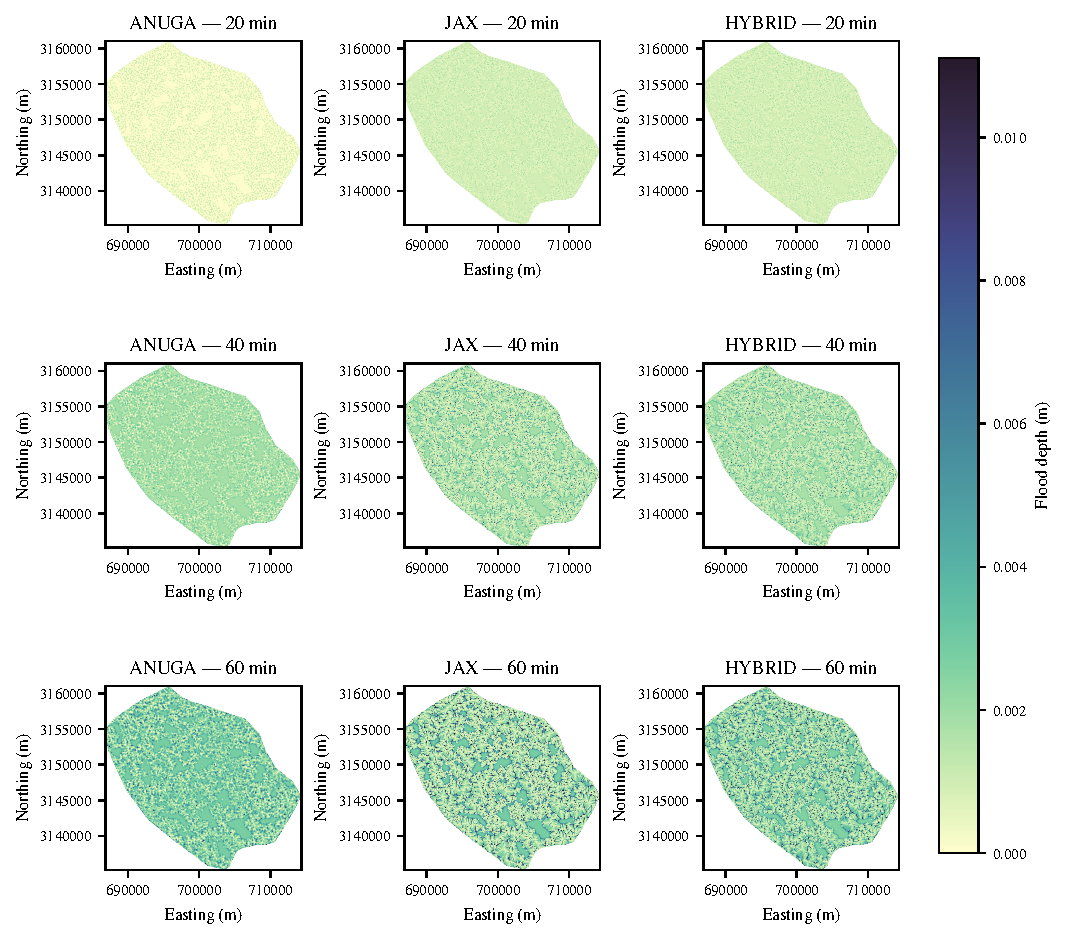
\includegraphics[width=\textwidth]{figures/flood_depth_comparison.pdf}
    \caption{ANUGA, pure-JAX, and hybrid flood-depth fields at 1200, 2400, and
    3600~s under the common reflective-boundary experiment.}
    \label{fig:flood-depth-comparison}
\end{figure}

\begin{figure}[htbp]
    \centering
    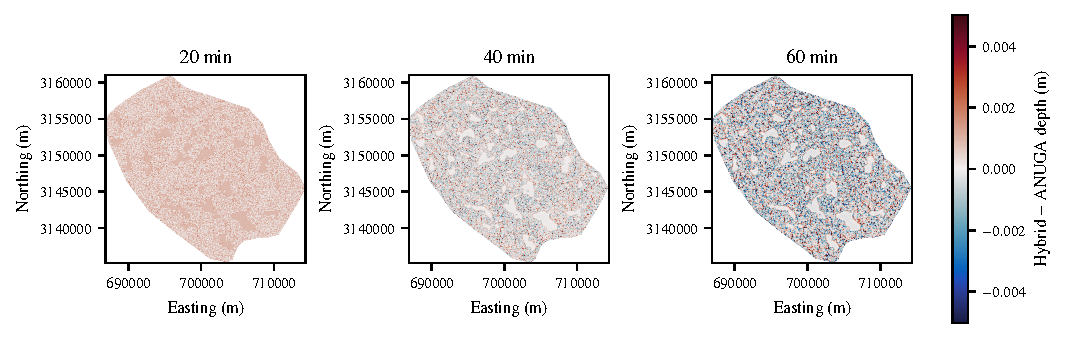
\includegraphics[width=0.9\textwidth]{figures/hybrid_depth_error.pdf}
    \caption{Hybrid-minus-ANUGA depth error at the configured key times.}
    \label{fig:hybrid-depth-error}
\end{figure}

\begin{figure}[htbp]
    \centering
    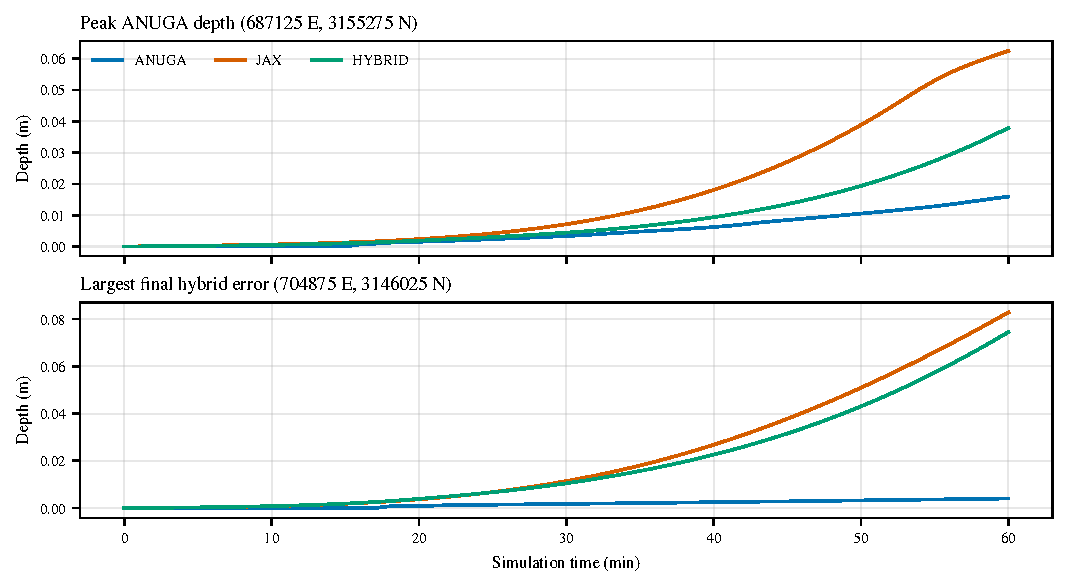
\includegraphics[width=0.9\textwidth]{figures/monitoring_point_hydrographs.pdf}
    \caption{Depth hydrographs at reproducibly selected monitoring locations
    for ANUGA, pure JAX, and the hybrid rollout.}
    \label{fig:monitoring-hydrographs}
\end{figure}

\subsection{GPU benchmark status}

No same-GPU JAX--PyTorch results are available.  The configured benchmark
correctly stopped because neither framework could access an NVIDIA device on
the execution host.  Therefore, no speedup, latency, compilation, or memory
result is reported.
